\documentclass[11pt]{article}
  \usepackage{pgfplots}
  \usepackage{graphicx}
  \usepackage{pdfpages}
  \pgfplotsset{compat=1.5.1} % 用来保证双 y 轴时两个 y 轴的 label 正确显示

  %%%%%%%%%%%%%%%%%%%%%%%%%%%%%%%%%%%%%%%%%
% Lachaise Assignment
% Structure Specification File
% Version 1.0 (26/6/2018)
%
% This template originates from:
% http://www.LaTeXTemplates.com
%
% Authors:
% Marion Lachaise & François Févotte
% Vel (vel@LaTeXTemplates.com)
%
% License:
% CC BY-NC-SA 3.0 (http://creativecommons.org/licenses/by-nc-sa/3.0/)
% 
%%%%%%%%%%%%%%%%%%%%%%%%%%%%%%%%%%%%%%%%%

%----------------------------------------------------------------------------------------
%	PACKAGES AND OTHER DOCUMENT CONFIGURATIONS
%----------------------------------------------------------------------------------------

\usepackage{amsmath,amsfonts,stmaryrd,amssymb} % Math packages

\usepackage{enumerate} % Custom item numbers for enumerations

\usepackage[ruled]{algorithm2e} % Algorithms

\usepackage[framemethod=tikz]{mdframed} % Allows defining custom boxed/framed environments

\definecolor{codegreen}{rgb}{0,0.2,0}
\definecolor{codegray}{rgb}{0.5,0.5,0.5}
\definecolor{codepurple}{rgb}{0.5,0.2,0.5}
\definecolor{codekeyword}{rgb}{0.5,0,0.22}

\usepackage{listings} % File listings, with syntax highlighting
\lstset{
	commentstyle=\color{codegreen},
	keywordstyle=\color{codekeyword},
	numberstyle=\tiny\color{codegray},
	stringstyle=\color{codepurple},
	basicstyle=\footnotesize,
	basicstyle=\ttfamily, % Typeset listings in monospace font
}

%----------------------------------------------------------------------------------------
%	DOCUMENT MARGINS
%----------------------------------------------------------------------------------------

\usepackage{geometry} % Required for adjusting page dimensions and margins

\geometry{
	paper=a4paper, % Paper size, change to letterpaper for US letter size
	top=2.5cm, % Top margin
	bottom=3cm, % Bottom margin
	left=2.5cm, % Left margin
	right=2.5cm, % Right margin
	headheight=14pt, % Header height
	footskip=1.5cm, % Space from the bottom margin to the baseline of the footer
	headsep=1.2cm, % Space from the top margin to the baseline of the header
	% showframe, % Uncomment to show how the type block is set on the page
}

%----------------------------------------------------------------------------------------
%	FONTS
%----------------------------------------------------------------------------------------

\usepackage[utf8]{inputenc} % Required for inputting international characters
\usepackage[T1]{fontenc} % Output font encoding for international characters

% \usepackage{XCharter} % Use the XCharter fonts\usepackage{XCharter} % Use the XCharter fonts

%----------------------------------------------------------------------------------------
%	COMMAND LINE ENVIRONMENT
%----------------------------------------------------------------------------------------

% Usage:
% \begin{commandline}
%	\begin{verbatim}
%		$ ls
%		
%		Applications	Desktop	...
%	\end{verbatim}
% \end{commandline}

\mdfdefinestyle{commandline}{
	innertopmargin=\baselineskip,
	leftmargin=0pt,
	rightmargin=0pt,
	innerleftmargin=5pt,
	middlelinecolor=black!50!white,
	middlelinewidth=2pt,
	frametitlerule=false,
	backgroundcolor=black!5!white,
	frametitle={Command Line},
	frametitlefont={\normalfont\sffamily\color{white}\hspace{-1em}},
	frametitlebackgroundcolor=black!50!white,
	nobreak,
	font=\small
}

% Define a custom environment for command-line snapshots
\newenvironment{commandline}{
	\medskip
	\begin{mdframed}[style=commandline]
}{
	\end{mdframed}
	\medskip
}

%----------------------------------------------------------------------------------------
%	FILE CONTENTS ENVIRONMENT
%----------------------------------------------------------------------------------------

% Usage:
% \begin{file}[optional filename, defaults to "File"]
%	File contents, for example, with a listings environment
% \end{file}

\mdfdefinestyle{file}{
	innertopmargin=\baselineskip,
	innerbottommargin=0.8\baselineskip,
	topline=false, bottomline=false,
	leftline=false, rightline=false,
	leftmargin=0cm,
	rightmargin=0cm,
	singleextra={%
		\draw[fill=black!10!white](P)++(0,-1.2em)rectangle(P-|O);
		\node[anchor=north west]
		at(P-|O){\ttfamily\mdfilename};
		%
		\def\l{3em}
		\draw(O-|P)++(-\l,0)--++(\l,\l)--(P)--(P-|O)--(O)--cycle;
		\draw(O-|P)++(-\l,0)--++(0,\l)--++(\l,0);
	},
	nobreak,
	font=\small
}

% Define a custom environment for file contents
\newenvironment{file}[1][File]{ % Set the default filename to "File"
	\medskip
	\newcommand{\mdfilename}{#1}
	\begin{mdframed}[style=file]
}{
	\end{mdframed}
	\medskip
}

%----------------------------------------------------------------------------------------
%	NUMBERED QUESTIONS ENVIRONMENT
%----------------------------------------------------------------------------------------

% Usage:
% \begin{question}[optional title]
%	Question contents
% \end{question}

\mdfdefinestyle{question}{
	innertopmargin=1.2\baselineskip,
	innerbottommargin=0.8\baselineskip,
	roundcorner=5pt,
	nobreak,
	singleextra={%
		\draw(P-|O)node[xshift=1em,anchor=west,fill=white,draw,rounded corners=5pt]{%
		Question \theQuestion\questionTitle};
	},
}

\newcounter{Question} % Stores the current question number that gets iterated with each new question

% Define a custom environment for numbered questions
\newenvironment{question}[1][\unskip]{
	\bigskip
	\stepcounter{Question}
	\newcommand{\questionTitle}{~#1}
	\begin{mdframed}[style=question]
}{
	\end{mdframed}
	\medskip
}

%----------------------------------------------------------------------------------------
%	WARNING TEXT ENVIRONMENT
%----------------------------------------------------------------------------------------

% Usage:
% \begin{warn}[optional title, defaults to "Warning:"]
%	Contents
% \end{warn}

\mdfdefinestyle{warning}{
	topline=false, bottomline=false,
	leftline=false, rightline=false,
	nobreak,
	singleextra={%
		\draw(P-|O)++(-0.5em,0)node(tmp1){};
		\draw(P-|O)++(0.5em,0)node(tmp2){};
		\fill[black,rotate around={45:(P-|O)}](tmp1)rectangle(tmp2);
		\node at(P-|O){\color{white}\scriptsize\bf !};
		\draw[very thick](P-|O)++(0,-1em)--(O);%--(O-|P);
	}
}

% Define a custom environment for warning text
\newenvironment{warn}[1][Warning:]{ % Set the default warning to "Warning:"
	\medskip
	\begin{mdframed}[style=warning]
		\noindent{\textbf{#1}}
}{
	\end{mdframed}
}

%----------------------------------------------------------------------------------------
%	INFORMATION ENVIRONMENT
%----------------------------------------------------------------------------------------

% Usage:
% \begin{info}[optional title, defaults to "Info:"]
% 	contents
% 	\end{info}

\mdfdefinestyle{info}{%
	topline=false, bottomline=false,
	leftline=false, rightline=false,
	nobreak,
	singleextra={%
		\fill[black](P-|O)circle[radius=0.4em];
		\node at(P-|O){\color{white}\scriptsize\bf i};
		\draw[very thick](P-|O)++(0,-0.8em)--(O);%--(O-|P);
	}
}

% Define a custom environment for information
\newenvironment{info}[1][Info:]{ % Set the default title to "Info:"
	\medskip
	\begin{mdframed}[style=info]
		\noindent{\textbf{#1}}
}{
	\end{mdframed}
}

\usepackage{fontspec}
\usepackage{indentfirst}
\usepackage{booktabs}
\usepackage{graphicx}
\usepackage{subfigure}
\usepackage{url}
\usepackage{flushend, cuted}
\usepackage{color}
\usepackage{enumitem} 

\XeTeXlinebreaklocale "zh"
\XeTeXlinebreakskip = 0pt plus 1pt
\setlength{\parindent}{2em} % 2em 代表首行缩进两个字符
% \linespread{1.2} % 设置行间距

\usepackage{tikz}
\usetikzlibrary{graphs, positioning, quotes, shapes.geometric} % Include the file specifying the document structure and custom commands

  % 如果提示没有字体,请修改此处的字体路径为当前编译文件的相对路径
  \setmainfont[ExternalLocation=../.template/]{STZHONGS.ttf}

  % 用于在代码内显示中文
  \usepackage{xeCJK}
  \setCJKmonofont[ExternalLocation=../.template/]{STZHONGS.ttf}

  \usepackage[font=small,labelfont=bf,tableposition=top]{caption}

  \DeclareCaptionLabelFormat{andtable}{#1~#2  \&  \tablename~\thetable}
  
  %----------------------------------------------------------------------------------------
  %	ASSIGNMENT INFORMATION
  %----------------------------------------------------------------------------------------
  
  \title{\Large 数据库原理及应用课程作业 \#1 \\
  \LARGE 思政资源数据库概念模型设计} % Title of the assignment
  
  \author{杨睿妮 \texttt{(2018011205014)} \\ \url{yangruinii@foxmail.com}} % Author name and email address
  
  \date{电子科技大学 --- \today} % University, school and/or department name(s) and a date
  
  %----------------------------------------------------------------------------------------
  
  \begin{document}
  
  \maketitle % Print the title

  \section{实验说明}
  \begin{itemize}
    \item 安装并学习使用 Power Designer 数据库辅助设计软件
    \item 使用 Power Designer 设计“课程思政”资源数据库概念模型 E-R 图
  \end{itemize}

  \section{实验原理}
  \begin{itemize}
    \item 数据库概念模式设计方法:自底向上、自顶向下和逐步扩张
    \item E-R表示方法:实体表示方法、属性表示方法、联系表示方法和数量关系表示方法
    \item E-R 图设计方法:设计局部 E-R 模式、全局 E-R 视图集成、全局 ER 集成过程中的冲突消除方法和消除冗余与优化方法
  \end{itemize}

  \section{实验环境}
  实验环境如表 \ref{tab:env} 所示。
  \begin{table}[h]
    \centering
    \caption{实验环境}
    \label{tab:env}
    \begin{tabular}{ll}
      \hline
      处理器 & lntel(R) Core(TM) i5-8300H CPU @2.30GHz \\
      \hline
      内存 & 16GB \\
      \hline
      软件 & Sybase PowerDesigner Version 16.5\\
      \hline
      操作系统 & Windows 10 \\
      \hline
    \end{tabular}
  \end{table}

  \section{实验步骤}
  \subsection{需求分析}

  本次实验建立的数据库需要满足以下业务需求:
  \begin{itemize}
    \item 每一份课程思政素材包含素材编号、标题、关键词、简介(摘要)、作者、素材来源、素材类别(如时政要闻、思想建设、人物楷模、时政专题、历史资料、新闻视频等)、采编者编号、采编者姓名、采编者所属单位、采编者邮箱、采编时间、点击阅读次数等;
    \item 需要建立树状结构学科目录,每个目录可以嵌套地包含下级子目录;
    \item 每一份课程思政素材可以归属到零个或多个学科目录,每个学科目录可以包含零个或多份课程思政素材;
    \item 每一份课程思政素材可以包含零个或多个多媒体文件,每个多媒体文件需要标注文件类别,以便调用播放软件;
    \item 设计并创建强实体模式:学科目录、思政素材、采编者;
    \item 设计并创建弱实体模式:多媒体文档;
    \item 设计并创建联系:学科目录内部层次之间的联系、思政素材与学科目录
    之间的联系、思政素材与采编者之间的联系、思政素材与多媒体文档之
    间的联系等

  \end{itemize}

  \subsection{设计并创建联系}

  根据需求,本次实验中的实体包括:学科、思政素材、多媒体素材以及采编者。每个实体的主键都是对应的Id。他们相互间的关系包括:思政素材(m)与多媒体素材(n)间的多对多关系、思政素材(m)与学科间(n)的多对多关系、思政素材(n)与学科(1)间的多对一关系、采编者(1)与多媒体素材(n)间的一对多关系以及采编者(1)与思政素材(n)间的一对多关系。

  由此得知,为了建立一对多的关系,“思政素材”实体中包含采编者的Id外键、“多媒体素材”实体中包含采编者的Id外键。为了建立多对多的关系,需要单独在关系表中插入两种实体的主键。

  此外,为了建立树状结构学科目录,并且便于后续在前端展示,在“学科”实体中添加“上级学科”属性,类型为 \verb|Integer|,用于标记该学科的上一级学科的Id,建立递归关系。

  \subsection{三种设计模型}
  利用Power Designer软件,搭建出概念设计模型后即可生成逻辑设计模型和物理设计模型。三种模型分别见图\ref{tab:CDMmodel}、\ref{tab:LDMmodel}和\ref{tab:PDMmodel}。三种模型的设计报告详见附录。

  \begin{figure}[h]
    \centering
    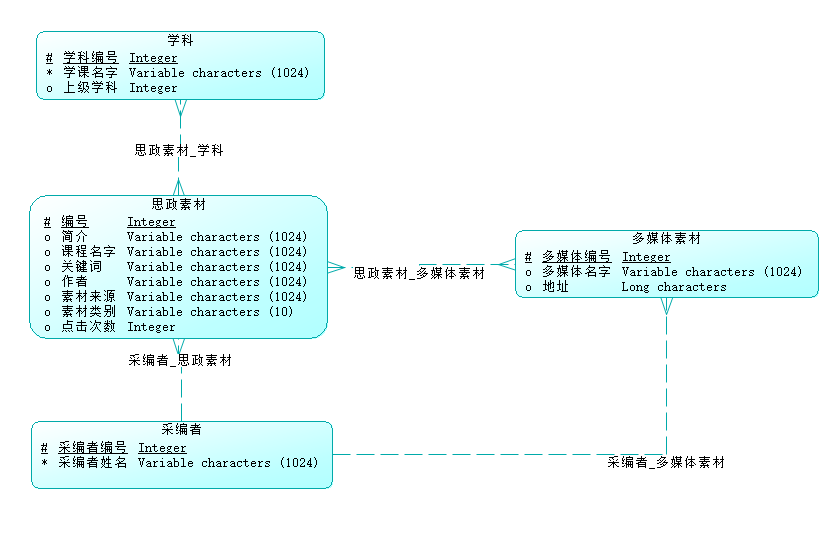
\includegraphics[width=\textwidth]{CDM模型.png}
    \caption{CDM模型}
    \label{tab:CDMmodel}
  \end{figure}

  \begin{figure}[p]
    \centering
    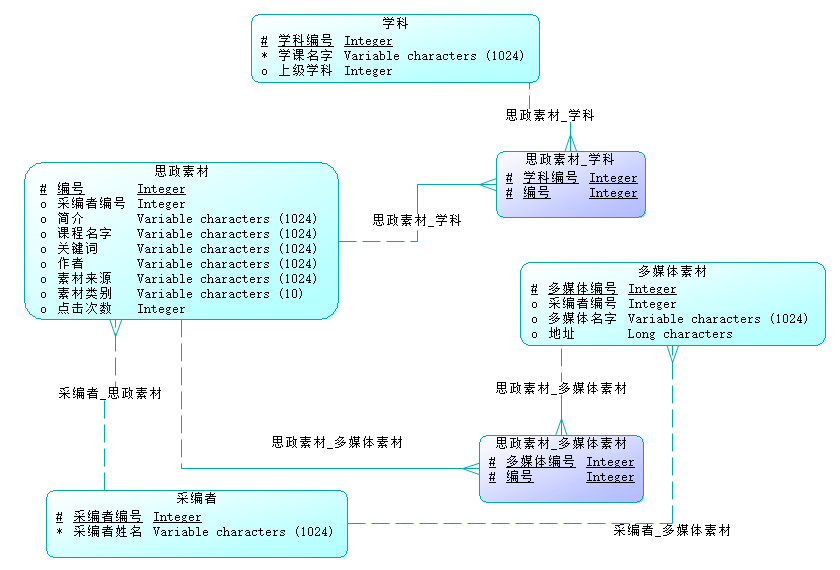
\includegraphics[width=0.8\textwidth]{LDM模型.png}
    \caption{LDM模型}
    \label{tab:LDMmodel}
  \end{figure}

  \begin{figure}[p]
    \centering
    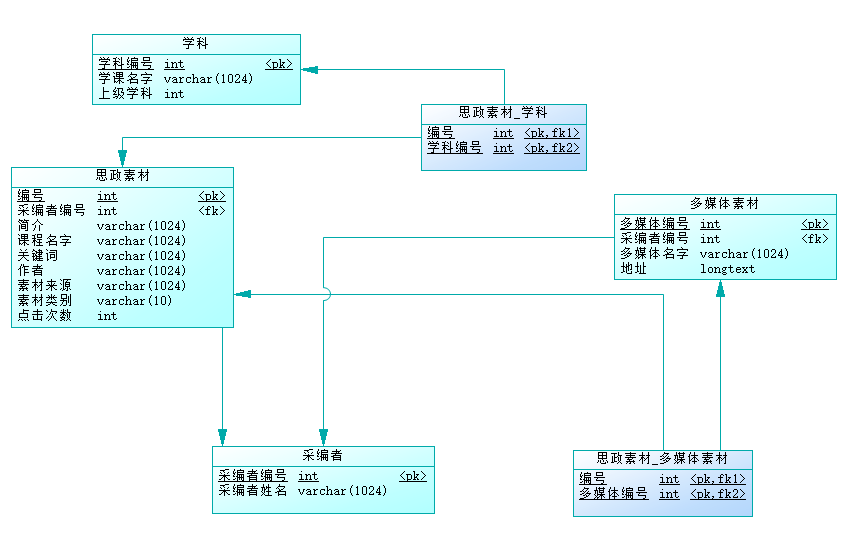
\includegraphics[width=0.8\textwidth]{PDM模型.png}
    \caption{PDM模型}
    \label{tab:PDMmodel}
  \end{figure}
  % 对照表见表 \ref{tab:comparison table}。
  % \begin{table}[h]
  %   \centering
  %   \caption{单词符号与种别对照表}
  %   \label{tab:comparison table}
  %   \begin{tabular}{ccccccccccc}
  %     \hline
  %     种别 & 01 & 02 & 03 & 04 & 05 & 06 & 07 & 08 & 09 & 10  \\
  %     \hline
  %     单词符号 & begin & end & integer & if & then & else & function & read & write & symbol \\
  %     \hline
  %     种别 & 11 & 12 & 13 & 14 & 15 & 16 & 17 & 18 & 19 & 20  \\
  %     \hline
  %     单词符号 & constant & = & <> & <= & < & >= & > & - & * & := \\
  %     \hline
  %     种别 & 21 & 22 & 23 & 24 & 25 \\
  %     \hline
  %     单词符号 & ( & ) & ; & EOLN & EOF \\
  %     \hline
  %   \end{tabular}
  % \end{table}
  \pagebreak
  \section{思考题}
  \pmb{Q:如何在 Power Designer 实现数据项(DataItem)的可复用?}

  “工具”菜单中有个选项“Model Option”,其中有一项设置,其默认选项是“Unique code”处于选中状态。PowerDesigner默认在CDM中不能存在相同名称的实体属性,这也是考虑到可能产生的一些如主键外键等名称冲突问题,但当我们进行实际数据库设计时,可能会多次使用相同数据项(DataItem)便于理解各实体。
  
  Unique code选项:data item是否必须有自己的代码。Allow reuse选项:选中表示允许一个data item作为多个entity的attribute,从而使这些attribute具有相同的name、data type以及部署以一个主键(这句不太理解,原文:and do not belong to a primary key)。当此项未被选中或者该attribute属于一个主键,那么data item不能被重用。这种情况下,如果Unique code选项被选中,一个具有相同名称但不同code的新的data item将被生成,否则一个具有相同名称和相同code的新的data item 将被创建。

  \pmb{Q:如何在 Power Designer 表示实体的侯选键?}

  候选键(Alternate Key)指一列或多列,表中每条记录的列值都是唯一的。每个候选键都在数据库中生成唯一索引或唯一约束。具体操作见图\ref{tab:AlternateKey}以及说明。
  \begin{itemize}
    \item[1.] 打开表的Keys选项卡,在空白的Name或Code栏中单击,系统自动增加一个新键。设置键的名称和代码
    \item[2.] 双击新键行的行首箭头,在打开的Key Properties(键属性)窗口中选择Columns选项卡,该选项卡列出了键包含的所有列
    \item[3.] 单击Add Columns图标,在窗口中列出了表中包含的所有列,选择一个或几个需要的列 
  \end{itemize}

  \begin{figure*}[h]
    \centering
    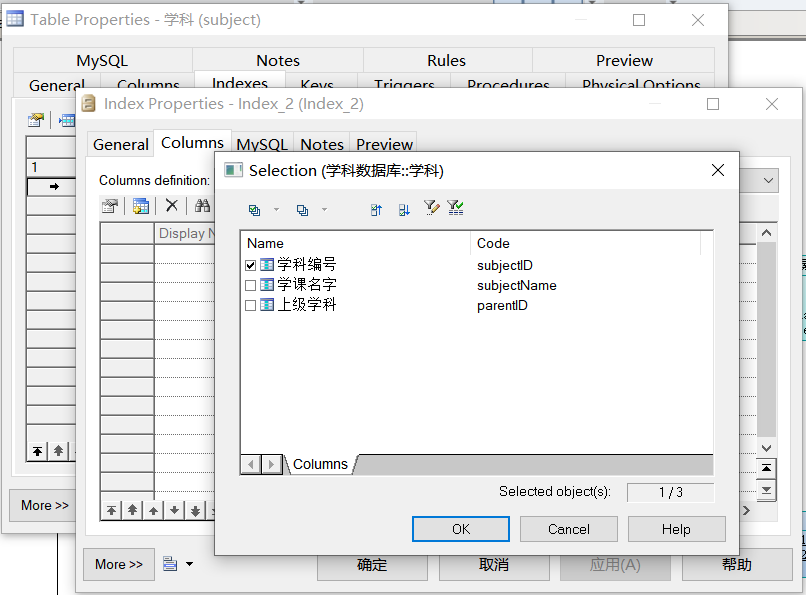
\includegraphics[width=0.6\textwidth]{候选键.png}
    \caption{候选键}
    \label{tab:AlternateKey}
  \end{figure*}

  \pmb{Q:如何在 Power Designer 自动生成概念设计报告?}

  选中Workspace中的概念模型 $\rightarrow$ 点击菜单栏中“Report” $\rightarrow$ 点击“Report Wizard...”即可按照提示生成相应报告。




% 含有三种错误的测试程序\verb|error-example-test.pas|如下:
% \lstinputlisting[]{../code/errot-example-test.pas}

% 含有三种错误的测试程序二元式输出文件\verb|error-example-out.dyd|如下:
% \lstinputlisting[]{../code/error-example-out.dyd}

% 含有三种错误的测试程序的错误输出文件\verb|error-example-error.err|如下:
% \lstinputlisting[]{../code/error-example-error.err}


  % \begin{enumerate}[itemindent=1em]
  %   \item 在确定作为筛的素数时,直接从 3 开始,从而跳过偶数;
  %   \item 在对素数的倍数进行标记时,直接跳过偶数;
  %   \item 在寻找下一个素数筛时,仅对奇数位标志进行检验;
  %   \item 在统计素数个数时,同样地只对奇数进行计算。
  % \end{enumerate}

  \pagebreak
  \section{实验总结}
  本次实验完成了思政资源数据库概念模型设计。在本次实验中学习使用了Power PowerDesigner软件,以课程思政资源数据库的建设任务为应用场景,运用所学习到的数据库建立以及E-R图绘制等相关知识,完成了数据库的建立工作。对于主键、外键以及实体间的各种关系有了更深刻的认识。
  
  \appendix
  % 附录代码开启行号
  \lstset{
	  numbers=left,
  }
  \pagebreak
  \section{附录:概念模型设计报告}
  \label{apd:CDM}
  \begin{figure*}[h]
    \centering
    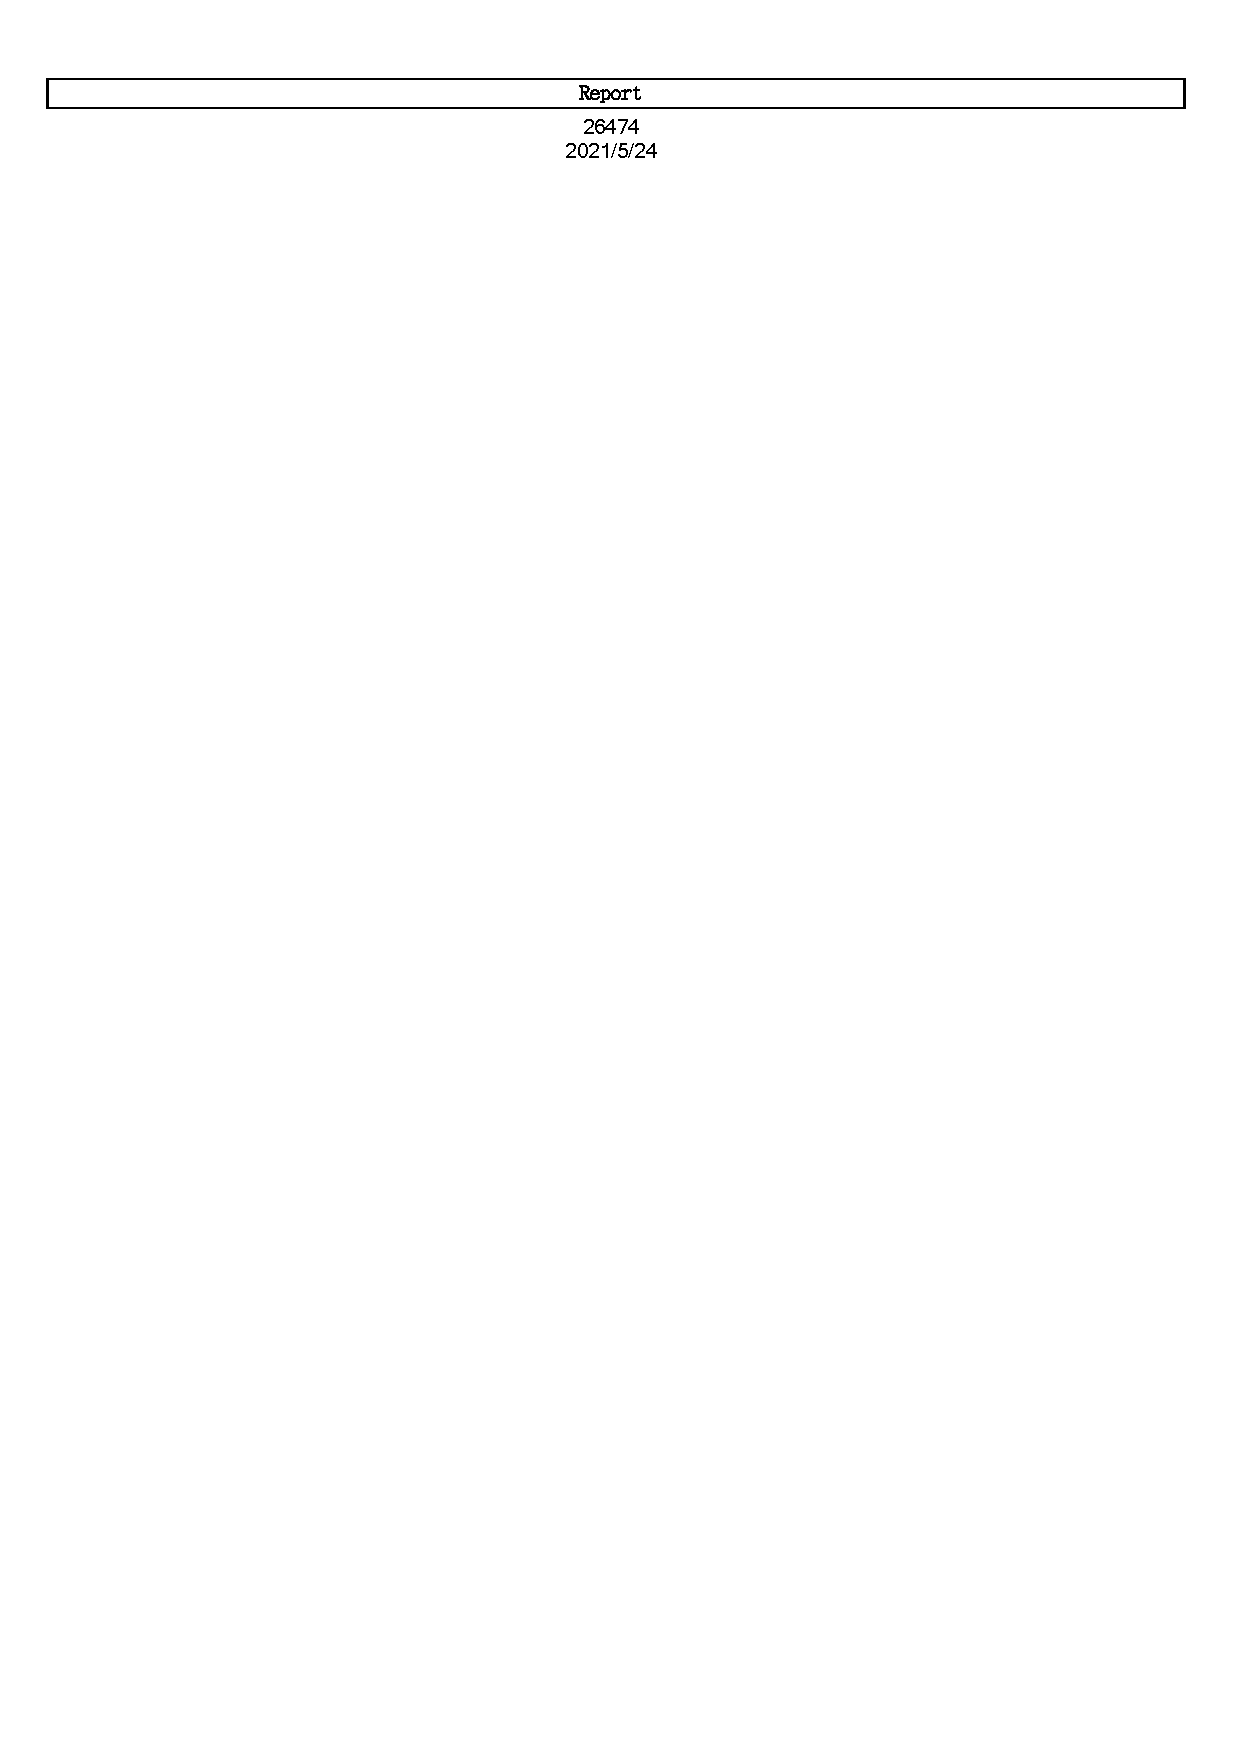
\includepdf[width=\textwidth, pages={1}]{../report/CDM.pdf}
  \end{figure*}
  \pagebreak
  \begin{figure*}[h]
    \centering
    \includepdf[width=\textwidth, pages={2}]{../report/CDM.pdf}
  \end{figure*}

  \pagebreak
  \begin{figure*}[h]
    \centering
    \includepdf[width=\textwidth, pages={3}]{../report/CDM.pdf}
  \end{figure*}
  \pagebreak
  \begin{figure*}[h]
    \centering
    \includepdf[width=\textwidth, pages={4}]{../report/CDM.pdf}
  \end{figure*}
  \pagebreak
  \begin{figure*}[h]
    \centering
    \includepdf[width=\textwidth, pages={5}]{../report/CDM.pdf}
  \end{figure*}
  \pagebreak
  \begin{figure*}[h]
    \centering
    \includepdf[width=\textwidth, pages={6}]{../report/CDM.pdf}
  \end{figure*}
  \pagebreak
  \begin{figure*}[h]
    \centering
    \includepdf[width=\textwidth, pages={7}]{../report/CDM.pdf}
  \end{figure*}
  \pagebreak
  \begin{figure*}[h]
    \centering
    \includepdf[width=\textwidth, pages={8}]{../report/CDM.pdf}
  \end{figure*}
  \pagebreak
  \begin{figure*}[h]
    \centering
    \includepdf[width=\textwidth, pages={9}]{../report/CDM.pdf}
  \end{figure*}
  \pagebreak
  \begin{figure*}[h]
    \centering
    \includepdf[width=\textwidth, pages={10}]{../report/CDM.pdf}
  \end{figure*}
  \pagebreak
  \begin{figure*}[h]
    \centering
    \includepdf[width=\textwidth, pages={11}]{../report/CDM.pdf}
  \end{figure*}
  \pagebreak
  \begin{figure*}[h]
    \centering
    \includepdf[width=\textwidth, pages={12}]{../report/CDM.pdf}
  \end{figure*}
  \pagebreak
  \begin{figure*}[h]
    \centering
    \includepdf[width=\textwidth, pages={13}]{../report/CDM.pdf}
  \end{figure*}
  \pagebreak
  \begin{figure*}[h]
    \centering
    \includepdf[width=\textwidth, pages={14}]{../report/CDM.pdf}
  \end{figure*}
  \pagebreak
  \begin{figure*}[h]
    \centering
    \includepdf[width=\textwidth, pages={15}]{../report/CDM.pdf}
  \end{figure*}
  \pagebreak
  \begin{figure*}[h]
    \centering
    \includepdf[width=\textwidth, pages={16}]{../report/CDM.pdf}
  \end{figure*}
  \pagebreak
  \begin{figure*}[h]
    \centering
    \includepdf[width=\textwidth, pages={17}]{../report/CDM.pdf}
  \end{figure*}
  \pagebreak
  \begin{figure*}[h]
    \centering
    \includepdf[width=\textwidth, pages={18}]{../report/CDM.pdf}
  \end{figure*}
  \pagebreak
  \begin{figure*}[h]
    \centering
    \includepdf[width=\textwidth, pages={19}]{../report/CDM.pdf}
  \end{figure*}
  \pagebreak
  \begin{figure*}[h]
    \centering
    \includepdf[width=\textwidth, pages={20}]{../report/CDM.pdf}
  \end{figure*}
  \pagebreak
  \begin{figure*}[h]
    \centering
    \includepdf[width=\textwidth, pages={21}]{../report/CDM.pdf}
  \end{figure*}
  \pagebreak
  \begin{figure*}[h]
    \centering
    \includepdf[width=\textwidth, pages={22}]{../report/CDM.pdf}
  \end{figure*}
  \pagebreak
  \begin{figure*}[h]
    \centering
    \includepdf[width=\textwidth, pages={23}]{../report/CDM.pdf}
  \end{figure*}
  \pagebreak
  \begin{figure*}[h]
    \centering
    \includepdf[width=\textwidth, pages={24}]{../report/CDM.pdf}
  \end{figure*}
  \pagebreak
  \begin{figure*}[h]
    \centering
    \includepdf[width=\textwidth, pages={25}]{../report/CDM.pdf}
  \end{figure*}
  \pagebreak
  \begin{figure*}[h]
    \centering
    \includepdf[width=\textwidth, pages={26}]{../report/CDM.pdf}
  \end{figure*}
  \pagebreak
  \begin{figure*}[h]
    \centering
    \includepdf[width=\textwidth, pages={27}]{../report/CDM.pdf}
  \end{figure*}
  
  \pagebreak
  \section{附录:物理模型设计报告}
  \label{apd:PDM}
  \begin{figure*}[h]
    \centering
    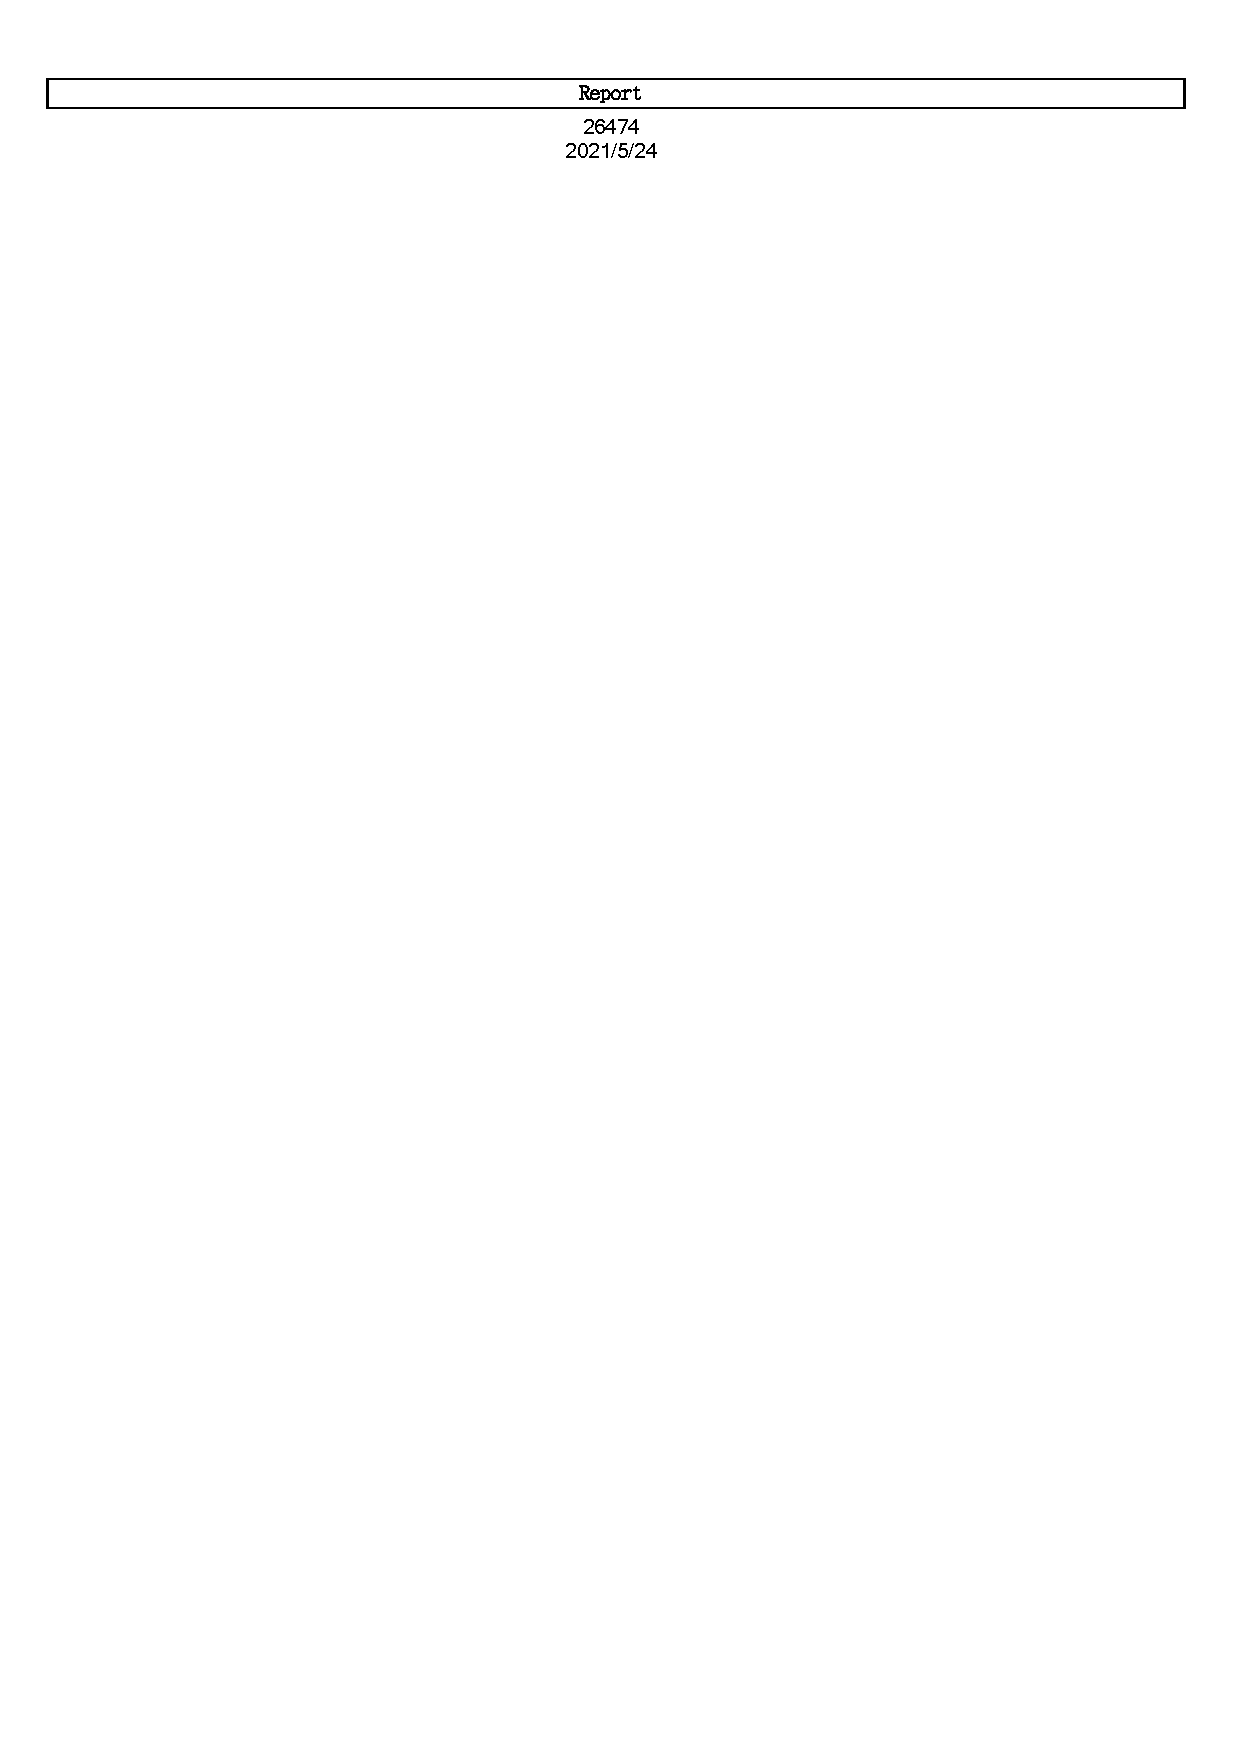
\includepdf[width=\textwidth, pages={1}]{../report/PDM.pdf}
  \end{figure*}
  \pagebreak
  \begin{figure*}[h]
    \centering
    \includepdf[width=\textwidth, pages={2}]{../report/PDM.pdf}
  \end{figure*}
  \pagebreak
  \begin{figure*}[h]
    \centering
    \includepdf[width=\textwidth, pages={3}]{../report/PDM.pdf}
  \end{figure*}
  \pagebreak
  \begin{figure*}[h]
    \centering
    \includepdf[width=\textwidth, pages={4}]{../report/PDM.pdf}
  \end{figure*}
  \pagebreak
  \begin{figure*}[h]
    \centering
    \includepdf[width=\textwidth, pages={5}]{../report/PDM.pdf}
  \end{figure*}
  \pagebreak
  \begin{figure*}[h]
    \centering
    \includepdf[width=\textwidth, pages={6}]{../report/PDM.pdf}
  \end{figure*}
  \pagebreak
  \begin{figure*}[h]
    \centering
    \includepdf[width=\textwidth, pages={7}]{../report/PDM.pdf}
  \end{figure*}
  \pagebreak
  \begin{figure*}[h]
    \centering
    \includepdf[width=\textwidth, pages={8}]{../report/PDM.pdf}
  \end{figure*}
  \pagebreak
  \begin{figure*}[h]
    \centering
    \includepdf[width=\textwidth, pages={9}]{../report/PDM.pdf}
  \end{figure*}
  \pagebreak
  \begin{figure*}[h]
    \centering
    \includepdf[width=\textwidth, pages={10}]{../report/PDM.pdf}
  \end{figure*}
  \pagebreak
  \begin{figure*}[h]
    \centering
    \includepdf[width=\textwidth, pages={11}]{../report/PDM.pdf}
  \end{figure*}
  \pagebreak
  \begin{figure*}[h]
    \centering
    \includepdf[width=\textwidth, pages={12}]{../report/PDM.pdf}
  \end{figure*}
  \pagebreak
  \begin{figure*}[h]
    \centering
    \includepdf[width=\textwidth, pages={13}]{../report/PDM.pdf}
  \end{figure*}
  \pagebreak
  \begin{figure*}[h]
    \centering
    \includepdf[width=\textwidth, pages={14}]{../report/PDM.pdf}
  \end{figure*}

  \pagebreak
  \section{附录:逻辑模型设计报告}
  \label{apd:LDM}
  \begin{figure*}[h]
    \centering
    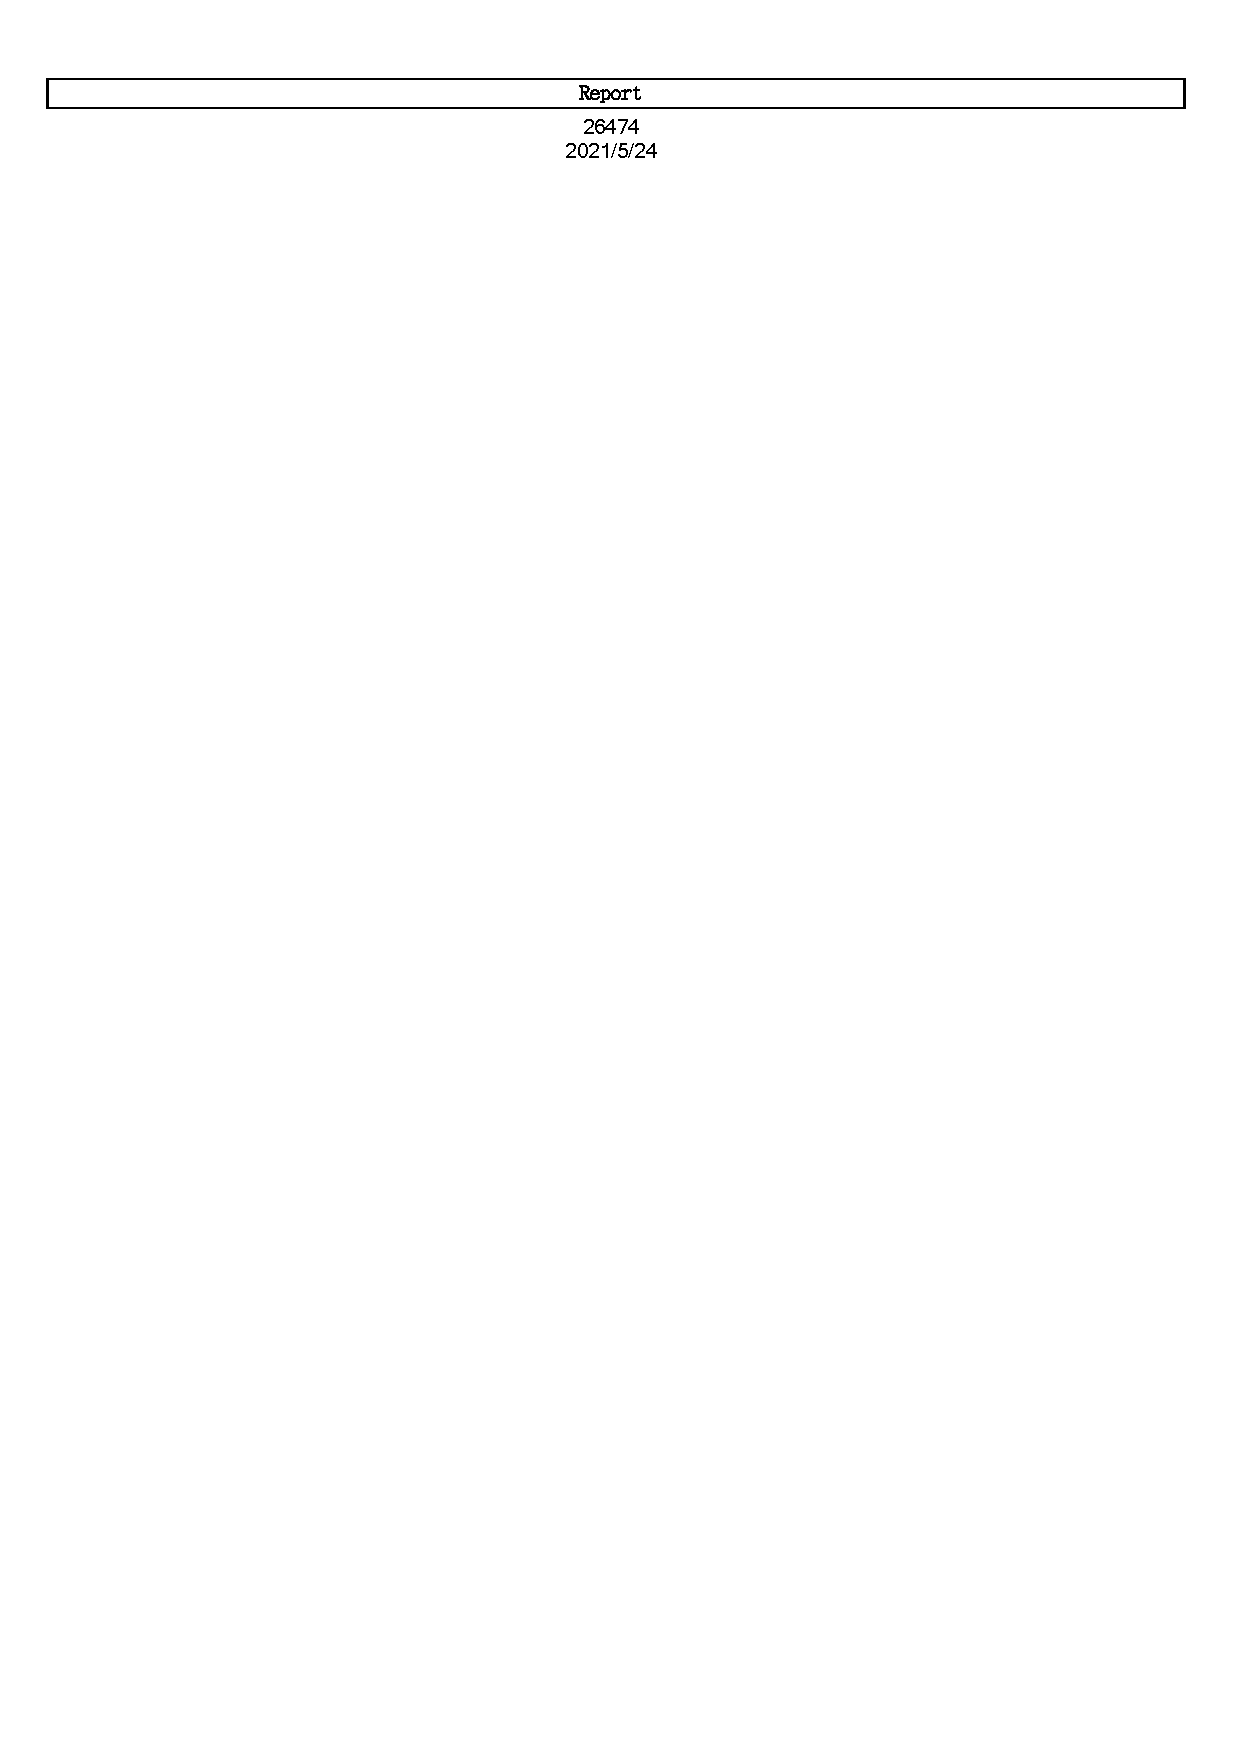
\includepdf[width=\textwidth, pages={1}]{../report/LDM.pdf}
  \end{figure*}
  \pagebreak
  \begin{figure*}[h]
    \centering
    \includepdf[width=\textwidth, pages={2}]{../report/LDM.pdf}
  \end{figure*}

  \pagebreak
  \begin{figure*}[h]
    \centering
    \includepdf[width=\textwidth, pages={3}]{../report/LDM.pdf}
  \end{figure*}
  \pagebreak
  \begin{figure*}[h]
    \centering
    \includepdf[width=\textwidth, pages={4}]{../report/LDM.pdf}
  \end{figure*}
  \pagebreak
  \begin{figure*}[h]
    \centering
    \includepdf[width=\textwidth, pages={5}]{../report/LDM.pdf}
  \end{figure*}
  \pagebreak
  \begin{figure*}[h]
    \centering
    \includepdf[width=\textwidth, pages={6}]{../report/LDM.pdf}
  \end{figure*}
  \pagebreak
  \begin{figure*}[h]
    \centering
    \includepdf[width=\textwidth, pages={7}]{../report/LDM.pdf}
  \end{figure*}
  \pagebreak
  \begin{figure*}[h]
    \centering
    \includepdf[width=\textwidth, pages={8}]{../report/LDM.pdf}
  \end{figure*}
  \pagebreak
  \begin{figure*}[h]
    \centering
    \includepdf[width=\textwidth, pages={9}]{../report/LDM.pdf}
  \end{figure*}
  \pagebreak
  \begin{figure*}[h]
    \centering
    \includepdf[width=\textwidth, pages={10}]{../report/LDM.pdf}
  \end{figure*}
  \pagebreak
  \begin{figure*}[h]
    \centering
    \includepdf[width=\textwidth, pages={11}]{../report/LDM.pdf}
  \end{figure*}
  \pagebreak
  \begin{figure*}[h]
    \centering
    \includepdf[width=\textwidth, pages={12}]{../report/LDM.pdf}
  \end{figure*}
  \pagebreak
  \begin{figure*}[h]
    \centering
    \includepdf[width=\textwidth, pages={13}]{../report/LDM.pdf}
  \end{figure*}
  \pagebreak
  \begin{figure*}[h]
    \centering
    \includepdf[width=\textwidth, pages={14}]{../report/LDM.pdf}
  \end{figure*}
  \pagebreak
  \begin{figure*}[h]
    \centering
    \includepdf[width=\textwidth, pages={15}]{../report/LDM.pdf}
  \end{figure*}
  


  % \section{附录:物理模型设计报告}
  % \label{apd:PDM}
  % \begin{figure*}[htp]
  %   \centering
  %   \includepdf[pages=-]{PDM.pdf}
  %   \label{pdf:PDM}
  % \end{figure*}

  % \section{附录:逻辑模型设计报告}
  % \label{apd:LDM}
  % \begin{figure*}[htp]
  %   \centering
  %   \includepdf[pages=-]{LDM.pdf}
  %   \label{pdf:LDM}
  % \end{figure*}
\end{document}